\documentclass[tikz,border=2mm]{standalone}

\begin{document}

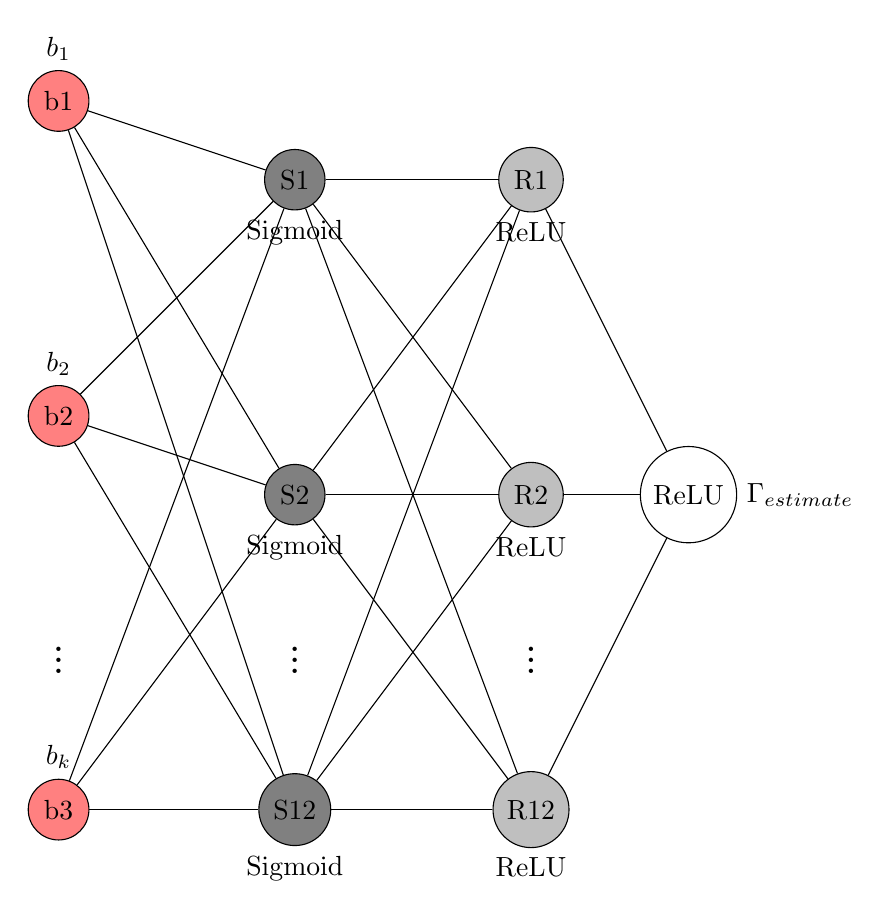
\begin{tikzpicture}
[   cnode/.style={draw=black,fill=#1,minimum width=5mm,circle},
]
%%%%%%%%%%%%%%%%%%%% OUTPUT LAYER %%%%%%%%%%%%%%%%%%%%%%%%%%%%%%%%%%%
    \node[cnode=white,label=0:$\Gamma_{estimate}$] (output) at (9,-7) {ReLU};


%%%%%%%%%%%%%%%%%%%% ReLU Layer %%%%%%%%%%%%%%%%%%%%%%%%%%%%%%%%%%%
    \node[cnode=black!25,label=-90:ReLU] (r1) at (7,-3) {R1};
    \node[cnode=black!25,label=-90:ReLU] (r2) at (7,-7) {R2};
    \node[cnode=black!25,label=-90:ReLU] (r3) at (7,-11) {R12};
    \node at (7,-9) {\textbf{$\vdots$}};
    \draw (r1) -- node[above,sloped,pos=0.3] {} (output);
    \draw (r2) -- node[above,sloped,pos=0.3] {} (output);
    \draw (r3) -- node[above,sloped,pos=0.3] {} (output);
    

%%%%%%%%%%%%%%%%%%%% Sigmoid Layer %%%%%%%%%%%%%%%%%%%%%%%%%%%%%%%%%%%
    \node[cnode=black!50,label=-90:Sigmoid] (s1) at (4,-3) {S1};
    \node[cnode=black!50,label=-90:Sigmoid] (s2) at (4,-7) {S2};
    \node[cnode=black!50,label=-90:Sigmoid] (s3) at (4,-11) {S12};
    \node at (4,-9) {\textbf{$\vdots$}};
    \draw (s1) -- node[above,sloped,pos=0.3] {} (r1);
    \draw (s1) -- node[above,sloped,pos=0.3] {} (r2);
    \draw (s1) -- node[above,sloped,pos=0.3] {} (r3);
    \draw (s2) -- node[above,sloped,pos=0.3] {} (r1);
    \draw (s2) -- node[above,sloped,pos=0.3] {} (r2);
    \draw (s2) -- node[above,sloped,pos=0.3] {} (r3);
    \draw (s3) -- node[above,sloped,pos=0.3] {} (r1);
    \draw (s3) -- node[above,sloped,pos=0.3] {} (r2);
    \draw (s3) -- node[above,sloped,pos=0.3] {} (r3);
    

    % \draw (b-\k) -- node[above,sloped,pos=0.3] {$\omega^{1}_{\pgfmathresult}$} (s1);
    % \draw (b-\k) -- node[above,sloped,pos=0.3] {$\omega^{2}_{\pgfmathresult}$} (s2);
    % \draw (b-\k) -- node[above,sloped,pos=0.3] {$\omega^{3}_{\pgfmathresult}$} (s3);

    \node at (1,-9) {\textbf{$\vdots$}};

    \foreach \k in {1,...,3}
    {   
        \pgfmathparse{\k<3 ? \k : "k"} % If x < 4 then give it its value, else give it the value N
        \node[cnode=red!50,label=90:$b_{\pgfmathresult}$] (b\k) at (1,{-\k-div(\k,3) - 3*\k + 2}) {b\k};
        \draw (b\k) -- node[above,sloped,pos=0.3] {} (s1);
        \draw (b\k) -- node[above,sloped,pos=0.3] {} (s2);
        \draw (b\k) -- node[above,sloped,pos=0.3] {} (s3);
    }
  


\end{tikzpicture}

\end{document}